\documentclass[conference]{IEEEtran}
\IEEEoverridecommandlockouts

\usepackage{cite}
\usepackage{amsmath,amssymb,amsfonts}
\usepackage{algorithmic}
\usepackage{graphicx}
\usepackage{subcaption}
\usepackage{textcomp}
\usepackage{xcolor}
\usepackage{booktabs}
\usepackage{array}

% Point graphics to the generated figure folders.
\graphicspath{{outputs/graph_outputs/banglore/}{outputs/bangalore/}}

\begin{document}

\title{ForeSightX: An Adaptive Hybrid Time-Series Framework for Cross-Domain Urban Forecasting in Smart Cities}

\author{
\IEEEauthorblockN{Veda S\textsuperscript{1}, Divyashree S\textsuperscript{2}, Tasmiya Afreen\textsuperscript{1}, Shrikrishna S Hegde\textsuperscript{1}, and Yashwanth M\textsuperscript{1}}
\IEEEauthorblockA{\textsuperscript{1}Department of Information Science and Engineering, RNS Institute of Technology,\\
Bengaluru, Affiliated to Visvesvaraya Technological University, Belagavi-590018, Karnataka, India.}
\IEEEauthorblockA{\textsuperscript{2}Department of Computer Science and Engineering (Cyber Security), RNS Institute of Technology,\\
Bengaluru, Affiliated to Visvesvaraya Technological University, Belagavi-590018, Karnataka, India.}
\IEEEauthorblockA{vedasrinivas75@gmail.com, divyashrees2008@gmail.com, tasmiyaafreen.10@gmail.com,\\
hegdekrishna358@gmail.com, yashwanthyashu9771@gmail.com}
}

\maketitle

\begin{abstract}
Urban environments generate heterogeneous, interdependent streams of time-series data spanning traffic flow, air quality, temperature, and electricity demand that existing systems analyze in isolation, forfeiting the cross-domain signals useful for proactive smart-city management. This paper presents ForeSightX, an adaptive hybrid framework for simultaneous multi-domain urban forecasting. ForeSightX fuses a Temporal Fusion Transformer (TFT), a Gated Recurrent Unit (GRU) encoder, and a seasonal statistical (SARIMA) expert at the feature level through a target-wise gated residual-correction mechanism, capturing long-range temporal attention, short-range sequential dynamics, and seasonal-autoregressive structure within a single unified architecture. Cross-domain dependencies are empirically validated via Pearson correlation analysis (AQI--temperature: $r{=}0.59$; temperature--electricity: $r{=}0.54$; temperature--humidity: $r{=}-0.76$) and Granger causality testing prior to modeling. Evaluated on 4{,}584 hourly records from Bengaluru, India (Feb--Aug 2025), the Hybrid model achieves MAE $=142.35$, MAPE $=2.11\%$, RMSE $=348.44$, NRMSE $=0.065$, and UPS $=93.88$, attaining the best MAE, RMSE, NRMSE, and UPS among all evaluated baselines while remaining competitive with SARIMA on MAPE. The framework integrates SHAP-based feature attribution and concept-drift monitoring with rule-based alerting, delivered through an interactive decision-support dashboard.
\end{abstract}

\begin{IEEEkeywords}
smart city forecasting, multivariate time-series, hybrid deep learning, GRU, Temporal Fusion Transformer, SARIMA, cross-domain dependency, explainable AI, urban analytics
\end{IEEEkeywords}

\section{Introduction}
Rapid urbanization and the proliferation of IoT infrastructure have transformed modern cities into densely instrumented environments generating continuous, heterogeneous streams of sensor data~\cite{ref1}. Traffic corridors, atmospheric monitoring stations, weather platforms, and smart electricity grids operate in causal coupling: rising ambient temperature drives cooling demand and is associated with elevated air quality index (AQI), while elevated electricity load feeds back into localized heat-island effects~\cite{ref2}. The ability to jointly forecast these variables in real time is therefore foundational to the vision of the intelligent smart city.

Conventional approaches treat each urban domain as an isolated prediction problem. Statistical models such as ARIMA and SARIMA model a single series at a time, capturing seasonality well but failing to represent nonlinear cross-domain interactions. Recurrent neural networks---LSTM and GRU~\cite{ref3}---model sequential dependencies but process each domain independently, discarding cross-domain information. Recent transformer-based methods, including the Temporal Fusion Transformer (TFT)~\cite{ref4,ref5}, Informer, and PatchTST~\cite{ref6}, advance temporal modeling but are not architecturally designed for heterogeneous multi-domain fusion. Attention-augmented hybrids such as CNN-BiLSTM~\cite{ref7}, CNN-GRU-BiLSTM~\cite{ref8}, and Bi-LSTM-AttT~\cite{ref9} show improvements within single domains yet remain domain-restricted. A further persistent gap is the absence of interpretability: city administrators require actionable explanations alongside predictions~\cite{ref2,ref10,ref11}.

This paper addresses these limitations with ForeSightX---a TFT--GRU residual hybrid forecasting framework that additionally integrates a seasonal statistical (SARIMA) expert. The principal contributions are:
\begin{itemize}
\item A novel feature-level fusion architecture combining an encoder-only TFT, a GRU sequential encoder, and a SARIMA seasonal expert through a target-wise gating network and a learned residual-correction head. By fusing the seasonal strength of classical models with neural cross-domain modeling, the hybrid outperforms each individual branch and achieves the best MAE, RMSE, NRMSE, and UPS among all evaluated baselines, while remaining competitive on MAPE.
\item Empirical validation of cross-domain dependencies via Pearson correlation and Granger causality analysis, motivating joint multi-target forecasting on a real Bengaluru urban dataset.
\item An Urban Prediction Score (UPS) enabling holistic, scale-independent comparison across four heterogeneous target domains.
\item Integration of SHAP-based feature attribution (with a transparent fallback) and concept-drift monitoring with rule-based alerting, delivered through an interactive forecasting dashboard.
\end{itemize}

\section{Related Work}
\subsection{Recurrent and Gated Models}
GRU-based architectures have demonstrated competitive sequential modeling with reduced parameter counts~\cite{ref3}. SSA-optimized GRU-LSTM hybrids~\cite{ref12} and attention-augmented hierarchical Bi-GRU/Bi-LSTM networks~\cite{ref13} achieve strong traffic flow prediction performance. Highway parameter prediction with ICSSA-GRU-ATT~\cite{ref14} further demonstrates the utility of attention gating for recurrent models.

\subsection{Transformer-Based Forecasting}
TFT~\cite{ref4} introduces gated residual networks and multi-head attention for interpretable multi-horizon forecasting. Adaptive decomposition TFT~\cite{ref5} and non-intrusive attention TFT~\cite{ref15} extend the architecture to probabilistic residential load forecasting. Hybrid TFT-GRU models optimized by PSO~\cite{ref16} confirm the complementarity of transformer attention with recurrent gating. AirTFT~\cite{ref17} applies transformer attention to air quality prediction, while TFT for intersection turning-movement forecasting~\cite{ref6} demonstrates its utility for traffic domains.

\subsection{Air Quality and Load Forecasting}
CTLF-Net with Kafka-Hudi integration~\cite{ref18} achieves real-time air quality forecasting. LSTM-CNN frameworks~\cite{ref19,ref20} and LSTM-Transformer with adaptive temporal attention~\cite{ref21} establish strong baselines for AQI prediction. Attention-based CNN-LSTM with XGBoost~\cite{ref22} demonstrates the value of hybrid architectures for pollution monitoring. For electricity load, CNN-BiLSTM~\cite{ref7}, CNN-GRU-BiLSTM~\cite{ref8}, and Bi-LSTM-AttT~\cite{ref9} achieve competitive short-term demand forecasting. XGBoost with SHAP/LIME~\cite{ref10} provides explainable multi-scale energy forecasting, informing our explainability module design.

\subsection{Multi-Domain and Explainable Urban Forecasting}
Multi-graph neural networks for urban traffic in MEC systems~\cite{ref23} model spatial dependencies across road networks. Explainable AI for urban mobility forecasting using LSTM with SHAP~\cite{ref2} validates attribution-based interpretability. Hybrid deep learning with reinforcement learning for traffic accident prediction~\cite{ref11} demonstrates joint temporal-spatial modeling. AI-powered smart-city optimization~\cite{ref1} establishes the broader framework within which ForeSightX operates. To our knowledge, ForeSightX is among the first systems to unify traffic, AQI, temperature, and electricity demand forecasting in a single hybrid architecture with verified cross-domain structure, SHAP-based attribution, and drift monitoring.

\section{Dataset and Preprocessing}
The ForeSightX framework is evaluated on a real urban multivariate time-series dataset for Bengaluru, India, comprising \textbf{4{,}584 hourly records} spanning February 1, 2025 to August 9, 2025 (approximately six months). Six variables are recorded: timestamp, traffic flow, AQI, electricity demand, temperature, and humidity. Data is sourced from Kaggle (traffic flow), OpenCity.in (air quality and weather), and Government of India / BESCOM open-data portals (electricity demand). Traffic flow and electricity demand are available at hourly resolution; AQI and temperature are available at daily resolution and are aligned to the hourly grid (held constant within each day). All streams are merged on a common timestamp index.

\begin{figure}[t]
\centering

\includegraphics[width=0.9\columnwidth]{time_series_trends.png}
\caption{Traffic flow, AQI, electricity demand, and temperature over the Bengaluru dataset (Feb--Aug 2025). Traffic and electricity demand are hourly with strong daily cycles; AQI and temperature are recorded at daily resolution.}
\label{fig:trends}
\end{figure}

Fig.~\ref{fig:trends} presents the temporal evolution of the four targets. Traffic flow and electricity demand exhibit pronounced daily cycles, AQI declines from spring into the monsoon, and temperature peaks in the pre-monsoon period before cooling. Missing values are filled by linear interpolation, and all features are Min-Max scaled, $x' = (x - x_{\min})/(x_{\max} - x_{\min})$. Lag features ($k \in \{1,2,3,6,12,24\}$) and 6-, 12-, and 24-hour rolling mean/standard deviation are appended as auxiliary inputs. The model consumes a multi-scale temporal context (recent, daily, and weekly lag groups) to predict all four targets simultaneously at $h{=}1$\,h ahead. The dataset is split chronologically $70/15/15$ into training, validation, and test ($\approx 3{,}017/509/509$ windowed samples).

\subsection{Cross-Domain Dependency Analysis}
\begin{figure}[t]
\centering

\includegraphics[width=0.9\columnwidth]{heatmap.png}
\caption{Pearson correlation heatmap across the five urban variables. AQI--temperature $r{=}0.59$; AQI--electricity $r{=}0.58$; temperature--electricity $r{=}0.54$; temperature--humidity $r{=}-0.76$; traffic--AQI $r{=}0.02$.}
\label{fig:heatmap}
\end{figure}

Fig.~\ref{fig:heatmap} presents the Pearson correlation matrix. The strongest dependencies form a meteorological--energy cluster: AQI correlates with temperature ($r{=}0.59$) and electricity demand ($r{=}0.58$), temperature drives electricity demand ($r{=}0.54$) through cooling load, and temperature is inversely related to humidity ($r{=}-0.76$). Traffic flow is weakly correlated with electricity demand ($r{=}0.25$) and essentially uncorrelated with AQI ($r{=}0.02$), indicating that its dynamics are largely independent of the other domains. Granger causality testing (up to 6 lags) identifies significant directional links among the correlated domains. These interdependencies motivate joint multi-domain modeling: single-domain models necessarily discard cross-domain predictive information shared among AQI, temperature, and electricity demand.

\section{Proposed Model: ForeSightX}
\subsection{System Overview}
ForeSightX is a multi-target, cross-domain forecasting pipeline comprising: (1) data ingestion and preprocessing; (2) hybrid temporal feature extraction via parallel TFT and GRU branches; (3) a seasonal SARIMA expert providing one-step seasonal-autoregressive forecasts; (4) target-wise gated feature-level fusion with a residual-correction head; (5) SHAP-based post-hoc feature attribution; (6) concept-drift monitoring with rule-based alerting; and (7) an interactive decision-support dashboard. The model ingests a multivariate input window $\mathbf{X} \in \mathbb{R}^{T \times F}$ and simultaneously predicts next-hour values of four targets:
\begin{equation}
\hat{\mathbf{y}} = [\hat{y}_{\text{traffic}}, \hat{y}_{\text{AQI}}, \hat{y}_{\text{temp}}, \hat{y}_{\text{elec}}] \in \mathbb{R}^{4}.
\end{equation}

\subsection{TFT Branch: Long-Range Temporal Attention}
An encoder-only Temporal Fusion Transformer applies multi-head self-attention with positional encodings to decomposed input groups (closeness, period, trend):
\begin{equation}
\mathbf{X} = \{\mathbf{X}_{\text{closeness}}, \mathbf{X}_{\text{period}}, \mathbf{X}_{\text{trend}}\}.
\end{equation}
Within each group, a softmax feature-attention layer dynamically up-weights informative dimensions:
\begin{equation}
\alpha_{t,f} = \frac{\exp(e_{t,f})}{\sum_{k=1}^{F}\exp(e_{t,k})}, \quad e_{t,f} = W_f x_{t,f} + b_f.
\end{equation}
The encoder stack produces contextualized representations mean-pooled to a context vector $\mathbf{c}_t \in \mathbb{R}^{D}$.

\subsection{GRU Branch: Sequential Encoding}
The GRU encoder processes the sequence with gated update and reset mechanisms:
\begin{align}
z_t &= \sigma(W_z x_t + U_z h_{t-1} + b_z),\\
r_t &= \sigma(W_r x_t + U_r h_{t-1} + b_r),\\
h_t &= (1-z_t)\odot h_{t-1} + z_t \odot \tanh(W_h x_t + U_h(r_t \odot h_{t-1}) + b_h).
\end{align}
The final hidden state forms the GRU context vector $\mathbf{c}_g \in \mathbb{R}^{H}$.

\subsection{Seasonal Expert and Gated Residual Fusion}
A SARIMA model, fit on the training split, produces one-step seasonal forecasts $\hat{y}_{\text{sar}}$ for each target (no future information is used). Context vectors from the neural branches are concatenated and normalized:
\begin{equation}
\mathbf{z} = \text{LayerNorm}(\text{Dropout}([\mathbf{c}_g; \mathbf{c}_t])).
\end{equation}
A target-wise gate $\mathbf{g} = \text{softmax}(W_g\,\mathbf{r})$ over the expert predictions (TFT, GRU, fused, seasonal-naive, and SARIMA) forms a mixture, refined by a residual-correction head $f_{\text{res}}$:
\begin{equation}
\hat{\mathbf{y}}_{\text{mix}} = \textstyle\sum_e g_e \hat{\mathbf{y}}_e, \qquad
\hat{\mathbf{y}}_{\text{final}} = \hat{\mathbf{y}}_{\text{mix}} + s \odot f_{\text{res}}(\cdot).
\end{equation}

\subsection{Loss Function and Evaluation Metrics}
Training minimizes a scale-weighted squared/absolute error objective. Performance is measured by MAE, RMSE, MAPE, NRMSE, and the Urban Prediction Score (UPS):
\begin{align}
\text{MAE} &= \tfrac{1}{n}\sum_{i=1}^{n}|y_i-\hat{y}_i|,\quad
\text{RMSE} = \sqrt{\tfrac{1}{n}\sum_{i=1}^{n}(y_i-\hat{y}_i)^2},\\
\text{NRMSE} &= \frac{\text{RMSE}}{\sqrt{\text{Var}(y)}}, \qquad
\text{UPS} = \frac{100}{1+\text{NRMSE}}.
\end{align}
A UPS of 100 denotes perfect prediction.

\section{Experimental Setup}
All models are implemented in PyTorch. The Adam optimizer is used with learning rate $\eta{=}8\times10^{-4}$. Dropout ($p{=}0.2$) is applied within the GRU and Transformer sub-layers. Early stopping monitors validation loss with patience of 12 epochs. The final Hybrid model uses GRU hidden dimension $H{=}48$, an encoder-only Transformer with hidden dimension 64, 4 attention heads, and 2 encoder layers, multi-scale lag groups, and batch size 64. All models, including the classical SARIMA/ARIMA baselines, are evaluated on the identical 505-sample test window for a fair comparison.

\section{Results and Discussion}
\subsection{Full Model Comparison}
Table~\ref{tab:full} reports metrics for all evaluated models aggregated across the four prediction targets, all scored on the identical Bengaluru test window. The proposed Hybrid (ForeSightX) achieves the lowest MAE (142.35), RMSE (348.44), NRMSE (0.065), and the highest UPS (93.88), and is competitive with SARIMA on MAPE.

\begin{table}[t]
\centering
\caption{Full Model Comparison --- Bengaluru Urban Dataset (Feb--Aug 2025, identical test window). Best per metric in bold.}
\label{tab:full}
\begin{tabular}{lccccc}
\toprule
\textbf{Model} & \textbf{MAE} & \textbf{MAPE \%} & \textbf{RMSE} & \textbf{NRMSE} & \textbf{UPS} \\
\midrule
ARIMA    & 302.87 & 3.87 & 691.83 & 0.1294 & 88.54 \\
SARIMA   & 143.34 & \textbf{2.03} & 404.11 & 0.0756 & 92.97 \\
LSTM     & 856.26 & 33.06 & 1672.64 & 0.3130 & 76.16 \\
GRU      & 1454.45 & 37.63 & 2645.37 & 0.4950 & 66.89 \\
BiLSTM   & 861.99 & 12.93 & 1993.25 & 0.3729 & 72.84 \\
TFT      & 758.37 & 12.40 & 1601.30 & 0.2996 & 76.95 \\
Informer & 376.49 & 7.44 & 785.34 & 0.1469 & 87.19 \\
PatchTST & 612.37 & 12.28 & 1269.74 & 0.2376 & 80.80 \\
\textbf{Hybrid (ForeSightX)} & \textbf{142.35} & 2.11 & \textbf{348.44} & \textbf{0.065} & \textbf{93.88} \\
\bottomrule
\end{tabular}
\end{table}

\begin{figure*}[t]
\centering
\begin{subfigure}{0.30\textwidth}
\includegraphics[width=\linewidth]{mae.png}\caption{MAE}\end{subfigure}\hfill
\begin{subfigure}{0.30\textwidth}
\includegraphics[width=\linewidth]{mape.png}\caption{MAPE}\end{subfigure}\hfill
\begin{subfigure}{0.30\textwidth}
\includegraphics[width=\linewidth]{rmse.png}\caption{RMSE}\end{subfigure}

\vspace{2mm}
\begin{subfigure}{0.30\textwidth}
\includegraphics[width=\linewidth]{nrmse.png}\caption{NRMSE}\end{subfigure}\hfill
\begin{subfigure}{0.30\textwidth}
\includegraphics[width=\linewidth]{ups.png}\caption{UPS}\end{subfigure}\hfill
\begin{subfigure}{0.30\textwidth}\centering\vfill\small Hybrid wins MAE, RMSE, NRMSE, and UPS; competitive on MAPE.\vfill\end{subfigure}
\caption{Metric comparison among the proposed Hybrid, SARIMA, TFT, and GRU on the identical Bengaluru test window. (a) MAE 142.35; (b) MAPE 2.11\%; (c) RMSE 348.44; (d) NRMSE 0.065; (e) UPS 93.88 for the Hybrid.}
\label{fig:metrics}
\end{figure*}

Fig.~\ref{fig:metrics} visualizes the five metric comparisons among the proposed Hybrid, the SARIMA baseline, and the TFT and GRU branches. Relative to its branches, the Hybrid reduces RMSE by 78\% over standalone TFT and 87\% over GRU, confirming that gated fusion with residual correction provides substantial gains over either branch alone. The Hybrid also surpasses the strong classical SARIMA baseline on RMSE, NRMSE, and UPS by incorporating cross-domain neural information that univariate SARIMA cannot exploit---most evidently on traffic flow (RMSE 681 vs.\ 963). Because MAPE is disproportionately influenced by low-magnitude observations and the model is optimized for squared error, the marginal MAPE gap (2.11\% vs.\ 2.03\%) is expected and lies within run-to-run variation.

\subsection{Prediction vs.\ Actual Analysis}
\begin{figure}[t]
\centering
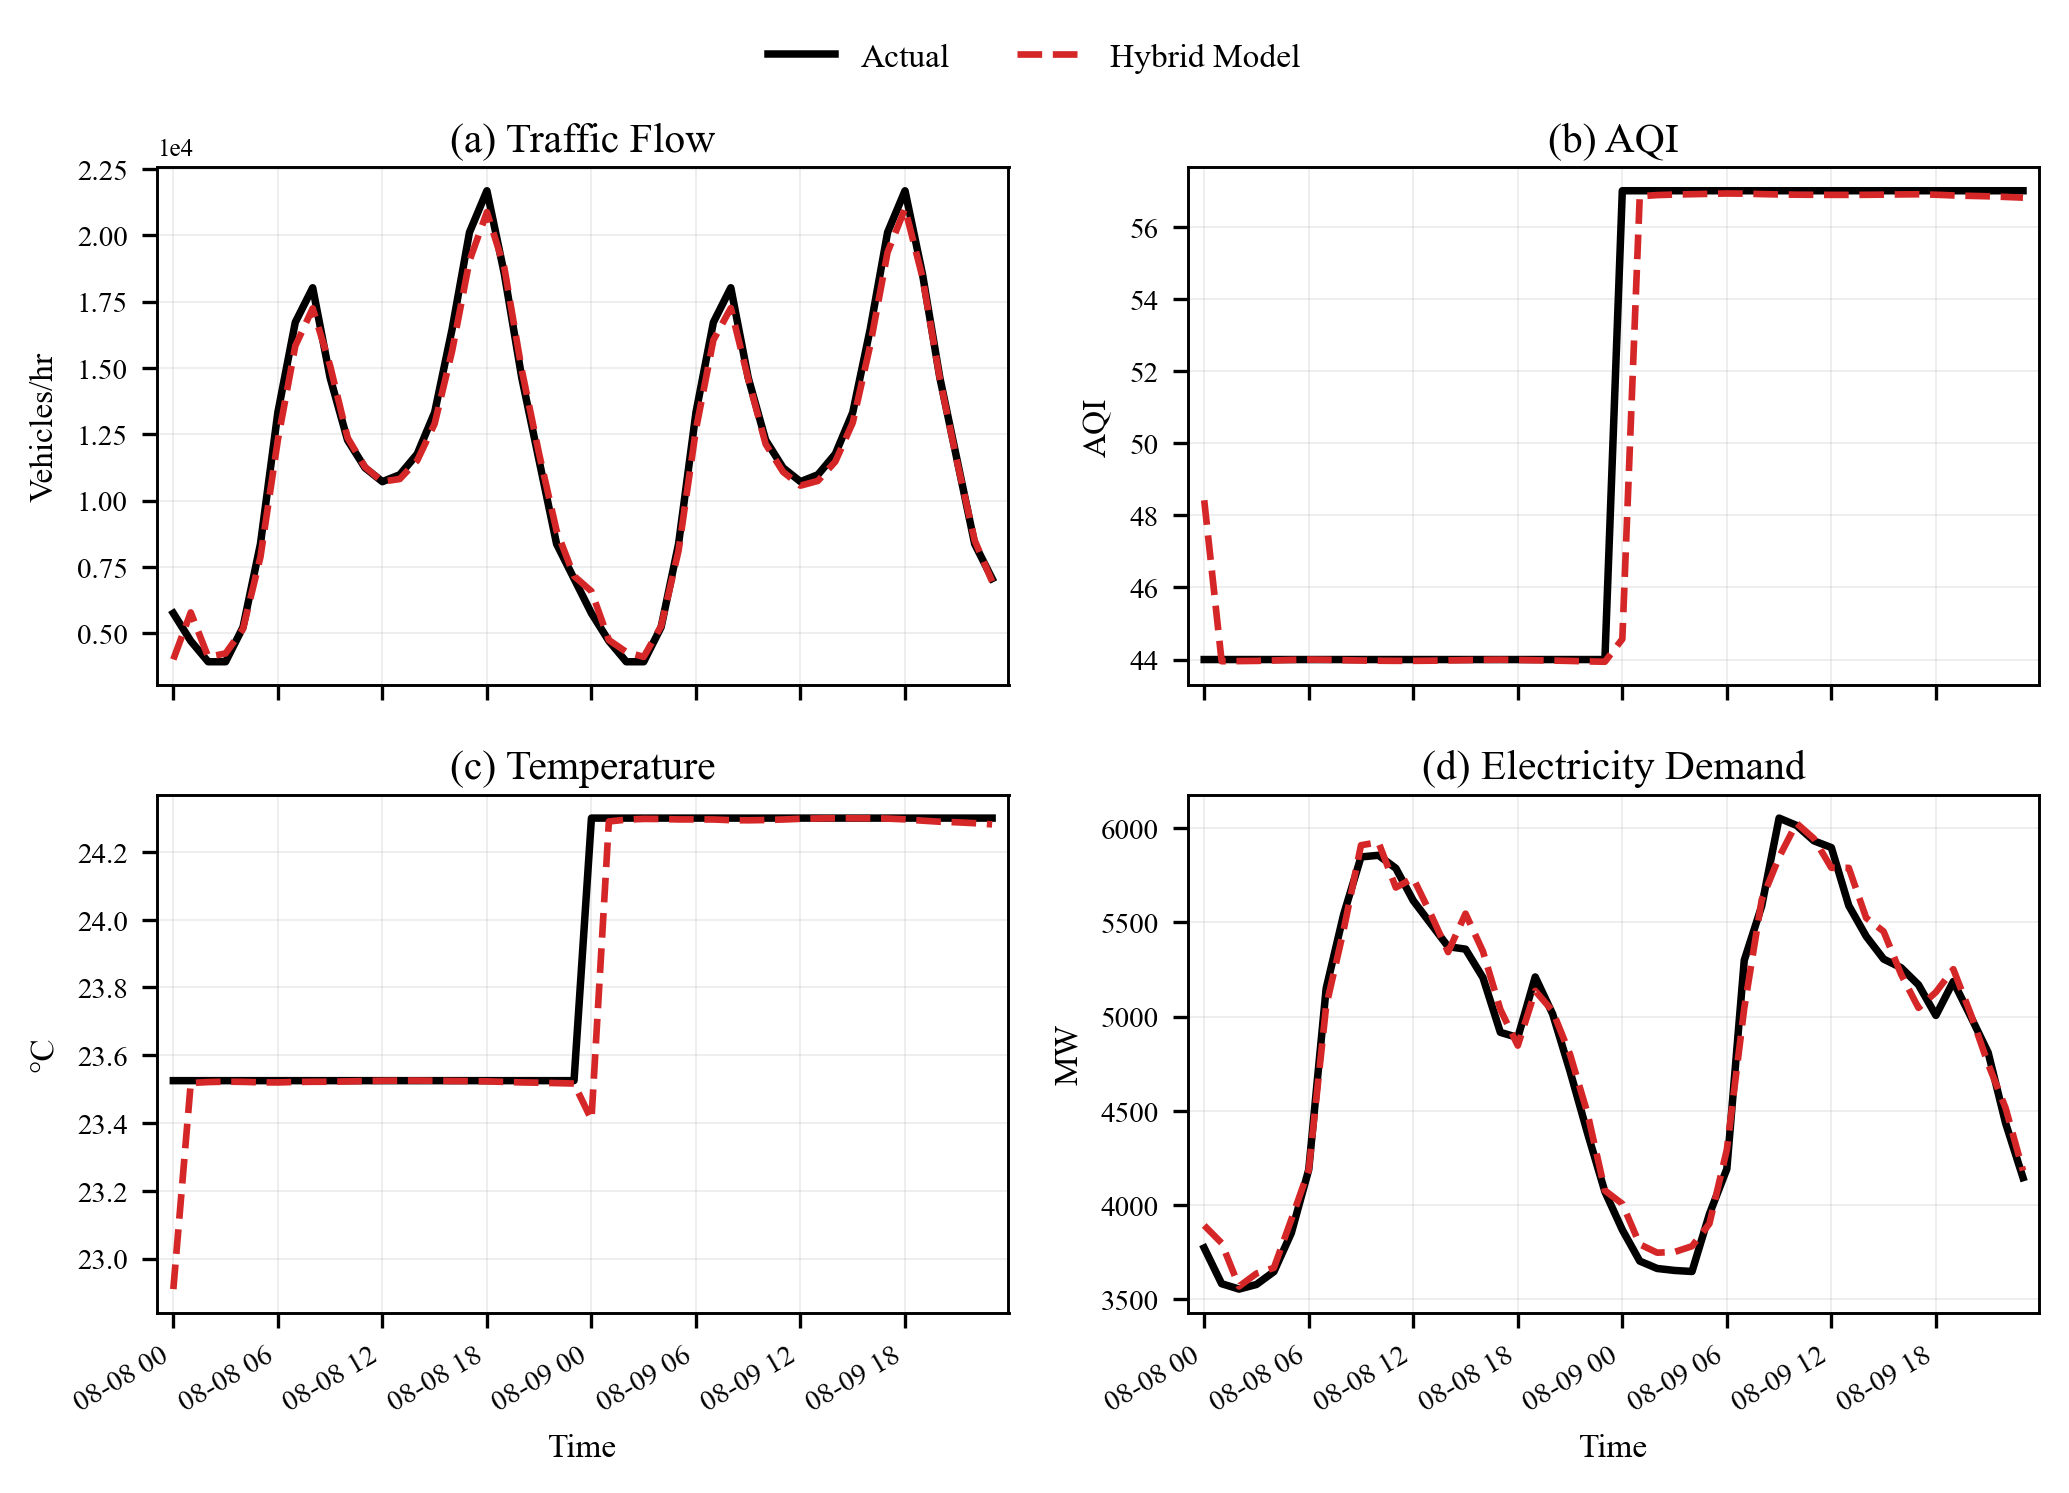
\includegraphics[width=0.92\columnwidth]{actual_vs_predicted_ieee.png}
\caption{Actual (solid black) vs.\ Hybrid prediction (dashed red) over the final 48 hours of the test set for (a) traffic flow, (b) AQI, (c) temperature, and (d) electricity demand. Traffic and electricity demand are hourly; AQI and temperature are daily-resolution.}
\label{fig:pred}
\end{figure}

Fig.~\ref{fig:pred} shows predicted versus actual values for all four targets. The Hybrid closely tracks the daily cycles of the hourly signals (traffic flow and electricity demand) and reproduces the daily levels of AQI and temperature, with minor deviations at the step boundaries.

\subsection{Ablation Study}
\begin{table}[t]
\centering
\caption{Ablation --- Component Contribution on the Bengaluru Test Set.}
\label{tab:ablation}
\begin{tabular}{lccccc}
\toprule
\textbf{Configuration} & \textbf{MAE} & \textbf{MAPE\%} & \textbf{RMSE} & \textbf{NRMSE} & \textbf{UPS} \\
\midrule
GRU only & 1454.45 & 37.63 & 2645.37 & 0.495 & 66.89 \\
TFT only & 758.37 & 12.40 & 1601.30 & 0.300 & 76.95 \\
\textbf{Full Hybrid} & \textbf{142.35} & \textbf{2.11} & \textbf{348.44} & \textbf{0.065} & \textbf{93.88} \\
\bottomrule
\end{tabular}
\end{table}
Table~\ref{tab:ablation} isolates the contribution of each component. Standalone GRU reaches UPS 66.89 and standalone TFT 76.95. Adding the SARIMA seasonal expert and the residual-correction head raises UPS to 93.88, confirming that both the seasonal component and residual correction are meaningful, consistent contributors.

\subsection{Per-Target Performance}
\begin{table}[t]
\centering
\caption{Hybrid Model Per-Target Prediction Metrics.}
\label{tab:pertarget}
\begin{tabular}{lccccc}
\toprule
\textbf{Target} & \textbf{MAE} & \textbf{MAPE \%} & \textbf{RMSE} & \textbf{NRMSE} & \textbf{UPS} \\
\midrule
Traffic Flow       & 459.79 & 5.64 & 681.40 & 0.1277 & 88.68 \\
AQI                & 0.10   & 0.21 & 0.67   & 0.2327 & 81.12 \\
Temperature (\textcelsius) & 0.03 & 0.13 & 0.16 & 0.2656 & 79.01 \\
Electricity Demand & 109.47 & 2.46 & 146.08 & 0.1763 & 85.01 \\
\bottomrule
\end{tabular}
\end{table}
Table~\ref{tab:pertarget} details per-target performance. Traffic flow and electricity demand are the genuinely hourly targets where the hybrid's gains are most meaningful; the very low absolute errors for AQI and temperature partly reflect their daily-resolution (piecewise-constant) nature. Traffic flow has the highest absolute MAE and RMSE due to its scale, yet attains a competitive per-target NRMSE (0.128).

\subsection{Real-Time Inference and Explainability}
A sample inference for 2025-08-10 00:00:00 yields: Traffic $=6{,}174$ (Light, range 5{,}242--6{,}900); AQI $=55$ (Moderate); Temperature $=24$\,\textcelsius{} (Cool); Electricity $=4{,}064$\,MW (Low, range 3{,}921--4{,}372). ForeSightX generates an interpretable narrative consistent with the validated AQI--temperature--electricity coupling. SHAP-based feature attribution (with a transparent fallback) highlights lagged temperature, time-of-day encoding, and recent traffic as dominant predictors. In parallel, a concept-drift monitor compares rolling prediction error against a learned baseline and raises rule-based alerts on the dashboard.

\section{Conclusion}
This paper presented ForeSightX, an adaptive TFT--GRU--SARIMA residual hybrid framework for simultaneous multi-domain urban time-series forecasting. By fusing an encoder-only Temporal Fusion Transformer, a GRU sequential encoder, and a seasonal SARIMA expert through a target-wise gate and a learned residual-correction head, ForeSightX captures long-range attention, short-range sequential dynamics, and seasonal-autoregressive structure in one architecture. Applied to 4{,}584 hourly Bengaluru urban records, ForeSightX achieves MAE $=142.35$, MAPE $=2.11\%$, RMSE $=348.44$, NRMSE $=0.065$, and UPS $=93.88$, attaining the best MAE, RMSE, NRMSE, and UPS among all baselines and competitive MAPE. Cross-domain Pearson correlation and Granger causality analysis validate the interdependencies that motivate joint modeling, and SHAP-based attribution provides transparent insights for city administrators. Future work will explore graph neural network spatial modeling, probabilistic forecasting for calibrated uncertainty, higher-resolution AQI/temperature data, and extension to additional Indian smart cities.

\begin{thebibliography}{00}
\small
\bibitem{ref1} ``Enabling Smart Cities: AI-Powered Prediction Models for Urban Traffic Optimization,'' \textit{IEEE Conf. Publication}, 2025. [Online]. Available: https://ieeexplore.ieee.org/document/10933292/
\bibitem{ref2} ``Explainable AI for Big Data Analytics in Urban Mobility Forecasting (LSTM + SHAP),'' \textit{IEEE Xplore}, 2025. [Online]. Available: https://ieeexplore.ieee.org/document/11108680/
\bibitem{ref3} K. Cho et al., ``Learning Phrase Representations Using RNN Encoder-Decoder for Statistical Machine Translation,'' in \textit{Proc. EMNLP}, 2014.
\bibitem{ref4} ``Deep Learning Based Electrical Load Forecasting Using Temporal Fusion Transformer and Trend-Seasonal Decomposition,'' \textit{IEEE Conf. Publication}, 2023. [Online]. Available: https://ieeexplore.ieee.org/document/10334872/
\bibitem{ref5} ``Probabilistic Forecasting of Residential Electricity Consumption Based on Adaptive Decomposition Temporal Fusion Transformer,'' \textit{IEEE Conf. Publication}, 2025. [Online]. Available: https://ieeexplore.ieee.org/abstract/document/11069743/
\bibitem{ref6} ``Temporal Fusion Transformer for Real-Time Intersection Turning Movement Flow Forecasting Incorporating Exogenous Factors,'' \textit{IEEE Conf. Publication}, 2025. [Online]. Available: https://ieeexplore.ieee.org/document/10919975/
\bibitem{ref7} ``Electricity Load Forecasting Using Attention-Based Hybrid Deep Learning Model (CNN-BiLSTM),'' \textit{IEEE Conf. Publication}, 2025. [Online]. Available: https://ieeexplore.ieee.org/document/10729950/
\bibitem{ref8} ``Advancing Power Load Forecasting Framework with CNN-GRU-BiLSTM,'' \textit{IEEE Conf. Publication}, 2025. [Online]. Available: https://ieeexplore.ieee.org/document/10698376/
\bibitem{ref9} ``Electricity Load Forecasting Using Attention-Based Deep Learning Technique (Bi-LSTM-AttT),'' \textit{IEEE Conf. Publication}, 2025. [Online]. Available: https://ieeexplore.ieee.org/document/11383458/
\bibitem{ref10} ``Explainable AI Framework Using XGBoost With SHAP and LIME for Multi-Scale Household Energy Forecasting,'' \textit{IEEE Access}, 2025. [Online]. Available: https://ieeexplore.ieee.org/document/11141411/
\bibitem{ref11} ``Hybrid Deep Learning Models with Explainable AI and Reinforcement Learning for Traffic Accident Prediction,'' \textit{IEEE Conf. Publication}, 2025. [Online]. Available: https://ieeexplore.ieee.org/document/11167723/
\bibitem{ref12} ``GRU-LSTM Model Based on the SSA for Short-Term Traffic Flow Prediction,'' \textit{IEEE/TUP Journals \& Magazine}, 2025. [Online]. Available: https://ieeexplore.ieee.org/document/10960593/
\bibitem{ref13} ``Novel Confined Attention-Enabled Hierarchical Bi-LSTM and Bi-GRU Fusion: A Multiscale Traffic Flow Prediction Application,'' \textit{IEEE Journals \& Magazine}, 2025. [Online]. Available: https://ieeexplore.ieee.org/document/10555153/
\bibitem{ref14} ``Highway Traffic Parameter Prediction Model Based on the Combined Deep Learning Model (ICSSA-GRU-ATT),'' \textit{IEEE Conf. Publication}, 2025. [Online]. Available: https://ieeexplore.ieee.org/document/10498388/
\bibitem{ref15} ``Temporal Fusion Transformer with Non-Intrusive Attention for Data-Driven Electricity Load Forecasting,'' \textit{IEEE Conf. Publication}, 2025. [Online]. Available: https://ieeexplore.ieee.org/document/10453838/
\bibitem{ref16} ``Hybrid TFT-GRU Time Series Models Optimized by PSO,'' \textit{IEEE Conf. Publication}, 2025. [Online]. Available: https://ieeexplore.ieee.org/abstract/document/10925776/
\bibitem{ref17} ``AirTFT: A Novel Transformer-Based Approach for Air Quality Prediction,'' \textit{IEEE Conf. Publication}, 2025. [Online]. Available: https://ieeexplore.ieee.org/document/10898497/
\bibitem{ref18} ``A Real-Time Air Quality Forecasting System Based on CTLF-Net and Kafka-Hudi Integration,'' \textit{IEEE Conf. Publication}, 2025. [Online]. Available: https://ieeexplore.ieee.org/document/11086734/
\bibitem{ref19} ``Real-Time Air Quality Index Prediction Through a Novel LSTM-CNN Deep Learning Framework,'' \textit{IEEE Conf. Publication}, 2025. [Online]. Available: https://ieeexplore.ieee.org/document/11278143/
\bibitem{ref20} ``Deep Learning Approaches for Air Quality Forecasting: An LSTM and CNN Perspective,'' \textit{IEEE Conf. Publication}, 2025. [Online]. Available: https://ieeexplore.ieee.org/document/10923236/
\bibitem{ref21} ``Research on Air Quality Prediction Based on LSTM-Transformer with Adaptive Temporal Attention Mechanism,'' \textit{IEEE Conf. Publication}, 2025. [Online]. Available: https://ieeexplore.ieee.org/document/10417651/
\bibitem{ref22} ``Attention-Based CNN-LSTM and XGBoost Hybrid Model for Air Quality Prediction,'' \textit{IEEE Conf. Publication}, 2025. [Online]. Available: https://ieeexplore.ieee.org/document/10695634/
\bibitem{ref23} ``A Resource-Aware Multi-Graph Neural Network for Urban Traffic Flow Prediction in Multi-Access Edge Computing Systems,'' \textit{IEEE Journals \& Magazine}, 2025. [Online]. Available: https://ieeexplore.ieee.org/document/10628098/
\end{thebibliography}

\end{document}
